% L9c logistic function figure: the probability of the label y = +1 against
% the score s = \hat{x}^T \theta, P = \sigma(2 \beta s) with
% \sigma(z) = 1/(1 + e^{-z}), for three inverse temperatures beta = 1/4, 1, 4.
% Every curve passes through 1/2 at s = 0, the decision boundary.
%
% Drawn on October 9, 2026 for the lecture's Logistic Regression section.
% Math uses the standard TeX fonts (no unicode-math), so \mathbf{\theta}
% renders as the same plain theta the notebook's math shows.
%
% The beta values are written into each plot expression. Do not introduce a
% pgfmath macro named \b, \a, or \fi (TeX primitives; see the L7c figure notes).
%
% The notebook SVG carries a dark palette added by theme_svg.py; keep new
% colors in that script's mapping when changing the palette here.
\documentclass[tikz,border=4pt]{standalone}
\usepackage[no-math]{fontspec}
\IfFontExistsTF{Arial}{\setsansfont{Arial}}{\setsansfont{TeX Gyre Heros}}
\renewcommand{\familydefault}{\sfdefault}
\usepackage{amsmath,amssymb}
\usetikzlibrary{arrows.meta}

% Same palette as the L9c gradient descent schematic.
\definecolor{vnink}{HTML}{202124}
\definecolor{gdblue}{HTML}{0091FF}
\definecolor{gdred}{HTML}{E02020}
\definecolor{gdgray}{HTML}{6D7278}

\begin{document}
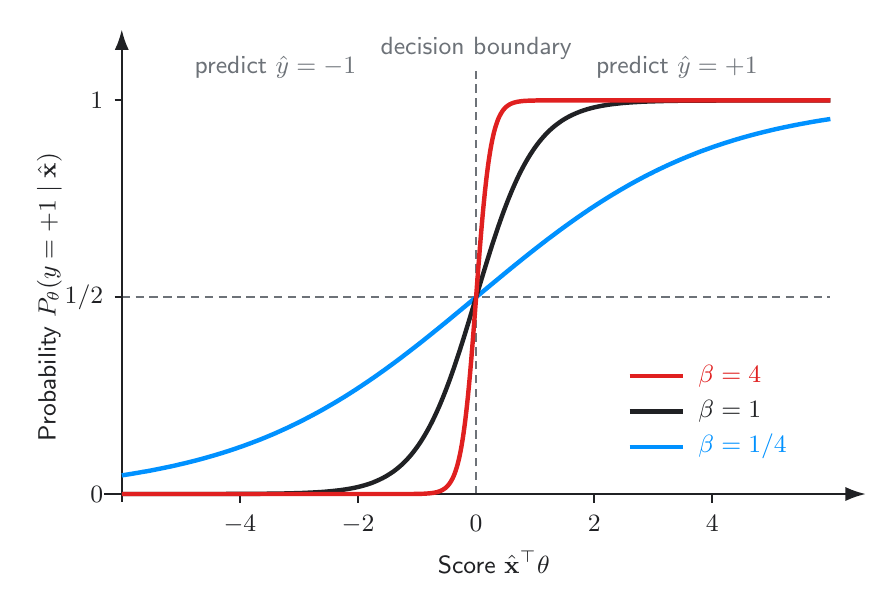
\begin{tikzpicture}[x=0.75cm, y=5cm, font=\sffamily\small, text=vnink,
    axis/.style={draw=vnink, line width=0.8pt, -{Latex[length=2.6mm, width=1.8mm]}},
    guide/.style={draw=gdgray, line width=0.8pt, dash pattern=on 3pt off 2pt},
    curve/.style={line width=1.6pt},
  ]
  % guides: probability 1/2 and the decision boundary s = 0
  \draw[guide] (-6, 0.5) -- (6, 0.5);
  \draw[guide] (0, 0) -- (0, 1.08);

  % axes
  \draw[axis] (-6.3, 0) -- (6.6, 0);
  \draw[axis] (-6, -0.02) -- (-6, 1.18);
  \foreach \y/\lab in {0/0, 0.5/{1/2}, 1/1} {
    \draw[vnink, line width=0.8pt] (-6.12, \y) -- (-6, \y);
    \node[anchor=east] at (-6.15, \y) {$\lab$};
  }
  \foreach \x in {-4, -2, 2, 4} {
    \draw[vnink, line width=0.8pt] (\x, 0) -- (\x, -0.024);
    \node[anchor=north] at (\x, -0.03) {$\x$};
  }
  \node[anchor=north] at (0, -0.03) {$0$};
  \node[anchor=north] at (0.3, -0.12) {Score $\hat{\mathbf{x}}^{\top}\mathbf{\theta}$};
  \node[rotate=90, anchor=south] at (-6.85, 0.5) {Probability $P_{\mathbf{\theta}}(y=+1\mid\hat{\mathbf{x}})$};

  % logistic curves sigma(2 beta s) for beta = 1/4, 1, 4. pgfmath overflows
  % above exp(9.7), so each curve is drawn in two halves that only take exp of
  % a non-positive number: sigma(z) = e^z/(1 + e^z) for z <= 0 and
  % 1/(1 + e^{-z}) for z >= 0.
  \draw[curve, gdblue] plot[domain=-6:0, samples=100, smooth] (\x, {exp(0.5*\x)/(1 + exp(0.5*\x))})
    -- plot[domain=0:6, samples=100, smooth] (\x, {1/(1 + exp(-0.5*\x))});
  \draw[curve, vnink] plot[domain=-6:0, samples=100, smooth] (\x, {exp(2*\x)/(1 + exp(2*\x))})
    -- plot[domain=0:6, samples=100, smooth] (\x, {1/(1 + exp(-2*\x))});
  \draw[curve, gdred] plot[domain=-6:0, samples=200, smooth] (\x, {exp(8*\x)/(1 + exp(8*\x))})
    -- plot[domain=0:6, samples=200, smooth] (\x, {1/(1 + exp(-8*\x))});

  % legend in the empty lower-right corner
  \draw[curve, gdred] (2.6, 0.30) -- (3.5, 0.30);
  \node[anchor=west, text=gdred] at (3.6, 0.30) {$\beta = 4$};
  \draw[curve, vnink] (2.6, 0.21) -- (3.5, 0.21);
  \node[anchor=west, text=vnink] at (3.6, 0.21) {$\beta = 1$};
  \draw[curve, gdblue] (2.6, 0.12) -- (3.5, 0.12);
  \node[anchor=west, text=gdblue] at (3.6, 0.12) {$\beta = 1/4$};

  % decision regions
  \node[anchor=south, text=gdgray] at (-3.4, 1.03) {predict $\hat{y} = -1$};
  \node[anchor=south, text=gdgray] at (3.4, 1.03) {predict $\hat{y} = +1$};
  \node[anchor=south, text=gdgray] at (0, 1.08) {decision boundary};
\end{tikzpicture}
\end{document}
